\documentclass[11pt]{article}

\usepackage[a4paper,margin=1in]{geometry}
\usepackage{amsmath,amssymb,bm,mathtools}
\usepackage{xcolor}
\usepackage{tikz}
\usepackage{placeins}
\usepackage[hidelinks]{hyperref}

\newcommand{\R}{\mathbb{R}}
\newcommand{\E}{\mathbb{E}}
\newcommand{\dd}{\mathop{}\!\mathrm{d}}
\newcommand{\supp}{\operatorname{supp}}
\newcommand{\KL}{\operatorname{KL}}
\newcommand{\Ent}{\operatorname{Ent}}

\title{Optimal Transport, Gradient Flow, and Schr\"odinger Bridges}
\author{}
\date{}

\begin{document}

\maketitle
\tableofcontents

\section{Moving mass at minimum cost}

Optimal transport asks how to rearrange one distribution into another while
paying as little transportation cost as possible. The source distribution
specifies where mass begins, the target distribution specifies where it must
end, and a cost function assigns a price to every possible movement.

The source and target spaces $\mathcal X$ and $\mathcal Y$ are subsets of
Euclidean spaces, with probability measures $\mu$ and $\nu$, respectively.
A measurable cost function
\begin{equation}
  c:\mathcal X\times\mathcal Y\to[0,\infty]
\end{equation}
assigns cost $c(x,y)$ to moving one unit of mass from $x$ to $y$. A common
choice is $c(x,y)=\lVert x-y\rVert^p$ for some $p\geq 1$.

Three related problems will be distinguished throughout the note. Optimal
transport finds a least-cost coupling between two prescribed endpoint
distributions. A Wasserstein gradient flow follows the steepest decrease of
an energy functional, using transport cost to measure the size of a step.
A Schr\"odinger bridge again fixes two endpoint distributions, but it selects
the most likely evolution relative to a prescribed reference distribution
over paths.

Consider source masses $0.6$ and $0.4$ at locations $x_1$ and $x_2$, and
target masses $0.5$ and $0.5$ at locations $y_1$ and $y_2$. The entry
$\pi_{ij}$ records the amount sent from $x_i$ to $y_j$. Conservation of mass
requires
\begin{equation}
  \begin{aligned}
    \pi_{11}+\pi_{12}&=0.6,
    &\pi_{21}+\pi_{22}&=0.4,\\
    \pi_{11}+\pi_{21}&=0.5,
    &\pi_{12}+\pi_{22}&=0.5,
  \end{aligned}
  \qquad \pi_{ij}\geq 0.
  \label{eq:two-location-constraints}
\end{equation}
If $C_{ij}=c(x_i,y_j)$, the total cost is
\begin{equation}
  \langle C,\pi\rangle
  =\sum_{i=1}^{2}\sum_{j=1}^{2}C_{ij}\pi_{ij}.
  \label{eq:discrete-cost}
\end{equation}
Optimal transport chooses the nonnegative matrix $\pi$ that satisfies
Eq.~\eqref{eq:two-location-constraints} and minimizes
Eq.~\eqref{eq:discrete-cost}. This small linear program already contains the
general structure of the Kantorovich formulation.

\section{Transport maps and transport plans}

There are two natural ways to describe the rearrangement. A transport map
sends each source point to one target point. A transport plan may split the
mass at a source point among several target points.

\subsection{The Monge problem}

A measurable map $T:\mathcal X\to\mathcal Y$ transports $\mu$ to $\nu$ if
the random variable $T(X)$ has distribution $\nu$ whenever $X$ has
distribution $\mu$. In measure notation this condition is
\begin{equation}
  T_{\#}\mu=\nu,
  \label{eq:pushforward}
\end{equation}
where $T_{\#}\mu$ is the pushforward of $\mu$ by $T$. Equivalently, for
every measurable set $B\subseteq\mathcal Y$,
\begin{equation}
  (T_{\#}\mu)(B)=\mu\bigl(T^{-1}(B)\bigr)=\nu(B).
\end{equation}
The Monge problem is
\begin{equation}
  \inf_{T:\,T_{\#}\mu=\nu}
  \int_{\mathcal X}c\bigl(x,T(x)\bigr)\,\dd\mu(x).
  \label{eq:monge}
\end{equation}

The map constraint can be too rigid. For example, one atom of mass cannot be
split by a deterministic map. If $\mu=\delta_0$ and
$\nu=\tfrac12\delta_{-1}+\tfrac12\delta_1$, no map $T$ can satisfy
$T_{\#}\mu=\nu$, because $T(0)$ is a single point.

\subsection{The Kantorovich relaxation}

A transport plan is a probability measure $\pi$ on
$\mathcal X\times\mathcal Y$. Its first marginal records the mass leaving
each source region, and its second marginal records the mass arriving in each
target region. The set of admissible couplings is
\begin{equation}
  \Pi(\mu,\nu)
  =\left\{\pi:
  \pi(A\times\mathcal Y)=\mu(A),\quad
  \pi(\mathcal X\times B)=\nu(B)
  \right\},
  \label{eq:couplings}
\end{equation}
where the equalities hold for all measurable
$A\subseteq\mathcal X$ and $B\subseteq\mathcal Y$. The Kantorovich problem
is
\begin{equation}
  \inf_{\pi\in\Pi(\mu,\nu)}
  \int_{\mathcal X\times\mathcal Y}c(x,y)\,\dd\pi(x,y).
  \label{eq:kantorovich}
\end{equation}

Every admissible map produces the plan
$\pi=(\operatorname{id},T)_{\#}\mu$, which is concentrated on the graph
$y=T(x)$. The converse need not hold because a general plan may distribute
mass from one $x$ over several values of $y$. Thus,
Eq.~\eqref{eq:kantorovich} is a relaxation of Eq.~\eqref{eq:monge}.

\section{The finite-dimensional linear program}

The discrete setting represents the two measures as
\begin{equation}
  \mu=\sum_{i=1}^{m}a_i\delta_{x_i},
  \qquad
  \nu=\sum_{j=1}^{n}b_j\delta_{y_j},
\end{equation}
where the nonnegative weights satisfy
$\sum_i a_i=\sum_j b_j=1$. The cost matrix has entries
$C_{ij}=c(x_i,y_j)$. A coupling is an $m\times n$ matrix whose entry
$\pi_{ij}$ is the mass transported from $x_i$ to $y_j$. The discrete
Kantorovich problem is
\begin{equation}
  \begin{aligned}
    \underset{\pi\in\R^{m\times n}}{\operatorname{minimize}}
    \quad &\sum_{i=1}^{m}\sum_{j=1}^{n}C_{ij}\pi_{ij}\\
    \text{subject to}\quad
    &\sum_{j=1}^{n}\pi_{ij}=a_i,
      &&i=1,\ldots,m,\\
    &\sum_{i=1}^{m}\pi_{ij}=b_j,
      &&j=1,\ldots,n,\\
    &\pi_{ij}\geq0.
  \end{aligned}
  \label{eq:discrete-ot}
\end{equation}
The row constraints preserve the source masses, and the column constraints
produce the target masses. Their total masses agree by assumption.

The constraints in Eq.~\eqref{eq:discrete-ot} define a feasible set
$\mathcal F$ containing many plans. The
optimization problem is to select the plan in $\mathcal F$ with the smallest
value of
\begin{equation}
  L(\pi)=\langle C,\pi\rangle
  =\sum_{i=1}^m\sum_{j=1}^n C_{ij}\pi_{ij},
  \qquad
  \bar\pi\in\operatorname*{argmin}_{\pi\in\mathcal F}L(\pi).
  \label{eq:transport-lp-objective}
\end{equation}
Let $\Delta$ be a change of the coupling matrix. It preserves both marginals
precisely when
\[
  \sum_j\Delta_{ij}=0,
  \qquad
  \sum_i\Delta_{ij}=0.
\]
There are $mn$ matrix elements and $m+n-1$ independent constraints, so the
space of such changes has dimension
\[
  mn-(m+n-1)=(m-1)(n-1).
\]

The basis is obtained directly. Let $\bm e_i$ denote a standard basis vector.
For every $i=1,\ldots,m-1$ and $j=1,\ldots,n-1$, define
\[
  D^{(ij)}
  =(\bm e_i-\bm e_m)(\bm e_j-\bm e_n)^{\mathsf T}.
\]
Each $D^{(ij)}$ has $+1$ at $(i,j)$ and $(m,n)$, $-1$ at $(i,n)$ and
$(m,j)$, and zero elsewhere. Thus every row and column sums to zero. For
$m=n=3$, the first basis matrix is
\begin{equation}
  D^{(11)}=
  \begin{bmatrix}
     1&0&-1\\
     0&0& 0\\
    -1&0& 1
  \end{bmatrix}.
  \label{eq:transport-four-entry-change}
\end{equation}

Generating all pairs $(i,j)$ produces exactly $(m-1)(n-1)$ basis matrices.
They are independent because $D^{(ij)}$ is the only one with a nonzero
$(i,j)$ entry in the upper-left $(m-1)\times(n-1)$ block. Every allowed
change has the unique expansion
\[
  \Delta
  =\sum_{i=1}^{m-1}\sum_{j=1}^{n-1}
   \Delta_{ij}D^{(ij)}.
\]
Indeed, the expansion reproduces the upper-left block of $\Delta$, while the
zero row and column sums uniquely determine its last row and last column.
This finite construction exhausts the basis; arbitrary coefficients exhaust
all marginal-preserving changes~\cite{warrington-2016}.

For any such $\Delta$, the plan $\pi+\theta\Delta$ preserves the marginal
constraints while it remains nonnegative. Its cost changes by
\begin{equation}
  L(\pi+\theta\Delta)-L(\pi)
  =\theta\langle C,\Delta\rangle.
  \label{eq:transport-four-entry-cost}
\end{equation}
If $\langle C,\Delta\rangle<0$, take the largest positive step that keeps
every matrix element nonnegative:
\begin{equation}
  \theta_{\max}
  =\min_{\Delta_{ij}<0}\frac{\pi_{ij}}{-\Delta_{ij}},
  \qquad
  \pi^{\mathrm{new}}_{ij}
  =\pi_{ij}+\theta_{\max}\Delta_{ij}.
  \label{eq:transport-update}
\end{equation}
The update lowers the cost and makes at least one matrix element zero. Repeat
the search from the new plan. If no feasible $\Delta$ satisfies
$\langle C,\Delta\rangle<0$, the current plan is optimal
~\cite{peyre-cuturi-2019}.

\section{Entropic transport and the Sinkhorn algorithm}

The linear program in Eq.~\eqref{eq:discrete-ot} becomes expensive when the
two supports are large. Entropic regularization changes the objective so that
the optimal coupling can be recovered by repeated matrix--vector products and
elementwise scaling~\cite{cuturi-2013,xie-2025}. For $\varepsilon>0$, define
\begin{equation}
  \mathcal L_\varepsilon(a,b;C)
  =\min_{\pi\in\Pi(a,b)}
  \left\{
    \sum_{i,j}C_{ij}\pi_{ij}
    +\varepsilon\sum_{i,j}\pi_{ij}(\log\pi_{ij}-1)
  \right\},
  \label{eq:entropic-ot}
\end{equation}
where $\Pi(a,b)$ is the matrix version of the coupling set in
Eq.~\eqref{eq:couplings}. The convention $0\log0=0$ is used. The entropy
term favors couplings that spread mass across more entries. When all
$a_i,b_j$ are positive and every $C_{ij}$ is finite, the objective is
strictly convex on the feasible set and has a unique positive optimizer.

\subsection{Why the optimizer is a scaled kernel}

Dual variables $f_i$ and $g_j$ enforce the row and column constraints, giving
the Lagrangian
\begin{equation}
  \begin{aligned}
  \mathcal L(\pi,f,g)
  ={}&\sum_{i,j}C_{ij}\pi_{ij}
     +\varepsilon\sum_{i,j}\pi_{ij}(\log\pi_{ij}-1)\\
    &+\sum_i f_i\left(a_i-\sum_j\pi_{ij}\right)
     +\sum_j g_j\left(b_j-\sum_i\pi_{ij}\right).
  \end{aligned}
  \label{eq:sinkhorn-lagrangian}
\end{equation}
Stationarity with respect to one entry gives
\begin{equation}
  C_{ij}+\varepsilon\log\pi_{ij}-f_i-g_j=0.
\end{equation}
Exponentiating this stationarity condition exposes the Gibbs kernel. Bars
denote converged dual potentials and scaling vectors:
\begin{equation}
  K_{ij}=\exp(-C_{ij}/\varepsilon),
  \qquad
  \bar u_i=\exp(\bar f_i/\varepsilon),
  \qquad
  \bar v_j=\exp(\bar g_j/\varepsilon).
  \label{eq:gibbs-kernel}
\end{equation}
The converged coupling has the component and matrix forms
\begin{equation}
  \bar\pi_{ij}=\bar u_iK_{ij}\bar v_j,
  \qquad
  \bar\pi=\operatorname{diag}(\bar u)K\operatorname{diag}(\bar v).
  \label{eq:sinkhorn-scaling}
\end{equation}
The first expression gives one entry. The second collects all $mn$ entries
into one matrix identity. Left multiplication by
$\operatorname{diag}(\bar u)$ scales row $i$ by $\bar u_i$, and right
multiplication by $\operatorname{diag}(\bar v)$ scales column $j$ by
$\bar v_j$. These identities apply only to the converged scaling vectors.

\subsection{Alternating marginal corrections}

At iteration $\ell$, the row correction chooses $u^{(\ell)}$ using
$v^{(\ell-1)}$. The following column correction chooses $v^{(\ell)}$ using
the new $u^{(\ell)}$. The enforced marginal equations are
\begin{equation}
  \begin{aligned}
    u_i^{(\ell)}[Kv^{(\ell-1)}]_i
      &=u_i^{(\ell)}\sum_{j=1}^{n}K_{ij}v_j^{(\ell-1)}=a_i,
      &&i=1,\ldots,m,\\
    v_j^{(\ell)}[K^\top u^{(\ell)}]_j
      &=v_j^{(\ell)}\sum_{i=1}^{m}K_{ij}u_i^{(\ell)}=b_j,
      &&j=1,\ldots,n.
  \end{aligned}
  \label{eq:sinkhorn-fixed-point}
\end{equation}
Here $Kv^{(\ell-1)}\in\R^m$ and $K^\top u^{(\ell)}\in\R^n$ are vectors.
Solving these two equations for the newly updated component gives
\begin{equation}
  \begin{aligned}
    u_i^{(\ell)}
      &=\frac{a_i}{[Kv^{(\ell-1)}]_i}
       =\frac{a_i}{\sum_{j=1}^{n}K_{ij}v_j^{(\ell-1)}},
       &&i=1,\ldots,m,\\
    v_j^{(\ell)}
      &=\frac{b_j}{[K^\top u^{(\ell)}]_j}
       =\frac{b_j}{\sum_{i=1}^{m}K_{ij}u_i^{(\ell)}},
       &&j=1,\ldots,n.
  \end{aligned}
  \label{eq:sinkhorn-updates}
\end{equation}
One may initialize $v^{(0)}$ to the all-ones vector. The first update makes every row sum equal
to $a_i$. The second makes every column sum equal to $b_j$, although it
generally disturbs the row sums again. Repetition drives both residuals to
zero under the usual positivity assumptions underlying matrix scaling
~\cite{sinkhorn-1964}.

For the two-location problem in Eq.~\eqref{eq:two-location-constraints}, the
same loop begins with the $2\times2$ matrix
$K_{ij}=\exp(-C_{ij}/\varepsilon)$. Each row rescaling supplies exactly
$0.6$ and $0.4$ units, and each column rescaling demands exactly $0.5$ and
$0.5$ units. The limit is the unique entropy-regularized version of the
coupling considered in Eq.~\eqref{eq:discrete-cost}.

A practical stopping rule measures both marginal errors, for example
\begin{equation}
  r(\pi)=
  \max\left\{
    \lVert\pi\boldsymbol{1}_n-a\rVert_1,
    \lVert\pi^\top\boldsymbol{1}_m-b\rVert_1
  \right\}.
  \label{eq:sinkhorn-residual}
\end{equation}
The algorithm stops when $r(\pi)$ is below a chosen numerical tolerance.
Checking the objective alone is insufficient because a nearly stationary
cost does not guarantee that both marginals are accurate.

\subsection{Log-domain stabilization}

Small $\varepsilon$ makes $K_{ij}=\exp(-C_{ij}/\varepsilon)$ extremely
small for expensive edges. Direct formation of $K$, $u$, and $v$ can then
underflow or overflow. The stable variables are the dual potentials
$f=\varepsilon\log u$ and $g=\varepsilon\log v$. Equation
~\eqref{eq:sinkhorn-updates} becomes
\begin{equation}
  \begin{aligned}
    f_i&=\varepsilon\log a_i
      -\varepsilon\log\sum_j
       \exp\left(\frac{g_j-C_{ij}}{\varepsilon}\right),\\
    g_j&=\varepsilon\log b_j
      -\varepsilon\log\sum_i
       \exp\left(\frac{f_i-C_{ij}}{\varepsilon}\right).
  \end{aligned}
  \label{eq:log-sinkhorn}
\end{equation}
Each logarithmic sum is evaluated with the log-sum-exp identity
\begin{equation}
  \log\sum_k e^{z_k}
  =z_{\max}+\log\sum_k e^{z_k-z_{\max}},
  \qquad z_{\max}=\max_k z_k.
  \label{eq:log-sum-exp}
\end{equation}
Every exponent on the right is at most zero. This removes the large positive
exponents that cause overflow.

When $z$ depends on trainable parameters, $z_{\max}$ also depends on them.
For the complete identity in Eq.~\eqref{eq:log-sum-exp}, this dependence
cancels exactly. With
\[
  w_k=\frac{e^{z_k-z_{\max}}}{\sum_r e^{z_r-z_{\max}}},
  \qquad \sum_k w_k=1,
\]
its differential is
\[
  \dd z_{\max}
  +\sum_k w_k(\dd z_k-\dd z_{\max})
  =\sum_k w_k\,\dd z_k.
\]
Thus a correctly implemented log-sum-exp has gradient
$\partial/\partial z_k=w_k$, including at the level of the full stabilized
expression. The cancellation must not be assumed for modified code. If
$z_{\max}$ is reused in another branch, detached in only one of its two
occurrences, rounded, or combined with clipping, its gradient contribution
need not cancel. Such code should retain the appropriate dependence on
$z_{\max}$ or supply a custom backward rule. A fused log-sum-exp primitive is
the safe choice when the complete identity is intended.

Log-sum-exp stabilization does not remove the conditioning problem
created by very small $\varepsilon$, so small-regularization computations may
still need more iterations or an $\varepsilon$-scaling schedule.

The parameter $\varepsilon$ controls a statistical and numerical tradeoff.
As $\varepsilon\downarrow0$, the regularized objective approaches the
unregularized transport objective and the coupling becomes more concentrated
on low-cost edges. At the same time, the kernel develops a larger dynamic
range and the scaling problem becomes harder. Larger $\varepsilon$ produces
a smoother coupling and a better-conditioned computation, but introduces
more entropic bias.

\subsection{Differentiating through the solution}

Let $P(a,b,C)=\bar\pi$ be the converged coupling. A general scalar loss may
depend on both the optimized transport value and the coupling:
\begin{equation}
  \mathcal J(a,b,C)
  =
  \Phi\!\left(
    \mathcal L_\varepsilon(a,b;C),
    P(a,b,C)
  \right).
  \label{eq:general-sinkhorn-loss}
\end{equation}
At the current solution, define
\begin{equation}
  G_{ij}=\frac{\partial\Phi}{\partial P_{ij}}.
  \label{eq:implicit-output-gradient}
\end{equation}
The total differential is
\begin{equation}
  \dd\mathcal J
  =\frac{\partial\Phi}{\partial\mathcal L_\varepsilon}
   \dd\mathcal L_\varepsilon
   +\langle G,\dd P\rangle.
  \label{eq:general-sinkhorn-chain-rule}
\end{equation}
The first term is obtained directly. The only issue considered below is how
to compute the second term, which requires the response $\dd P$ of the
converged plan.
The stationarity equation and the two marginal equations are
\begin{equation}
  C_{ij}+\varepsilon\log P_{ij}-\bar f_i-\bar g_j=0,
  \qquad
  P\boldsymbol 1_n=a,
  \qquad
  P^\top\boldsymbol 1_m=b.
  \label{eq:implicit-forward-equations}
\end{equation}
Within the inner Sinkhorn optimization, $a$, $b$, and $C$ are held fixed
while $P$, $\bar f$, and $\bar g$ are solved. In the outer differentiation,
an input may vary through an upstream parameter $\theta$; for example,
$C=C(\theta)$ gives
$\dd C=(\partial C/\partial\theta)\dd\theta$. Thus \emph{fixed} refers only
to the inner optimization. If $a$ and $b$ are fixed ensemble weights, set
$\dd a=\dd b=0$ while retaining $\dd C$. Differentiating the first equation
gives
\begin{equation}
  \dd C_{ij}
  +\varepsilon\frac{\dd P_{ij}}{P_{ij}}
  -\dd\bar f_i-\dd\bar g_j=0
  \qquad\Longrightarrow\qquad
  \dd P_{ij}
  =\frac{P_{ij}}{\varepsilon}
    (\dd\bar f_i+\dd\bar g_j-\dd C_{ij}).
  \label{eq:implicit-sinkhorn-differential}
\end{equation}
Equation~\eqref{eq:implicit-sinkhorn-differential} is already the desired
entrywise response $\dd P_{ij}$, except that $\dd\bar f$ and $\dd\bar g$ are
still unknown. They are fixed by differentiating the two marginal
constraints:
\begin{equation}
  \sum_j\dd P_{ij}=\dd a_i,
  \qquad
  \sum_i\dd P_{ij}=\dd b_j.
  \label{eq:differentiated-marginal-constraints}
\end{equation}
Substituting Eq.~\eqref{eq:implicit-sinkhorn-differential} into these two
relations gives
\begin{equation}
  \varepsilon\dd a_i
  =a_i\dd\bar f_i+\sum_jP_{ij}\dd\bar g_j
   -\sum_jP_{ij}\dd C_{ij},
  \qquad
  \varepsilon\dd b_j
  =\sum_iP_{ij}\dd\bar f_i+b_j\dd\bar g_j
   -\sum_iP_{ij}\dd C_{ij}.
  \label{eq:differentiated-marginals}
\end{equation}
Consider the quadratic cost
$C_{ij}=\frac12\lVert x_i-y_j\rVert^2$ and ask how the converged plan changes
when one source position $x_k$ changes. The weights and all other positions
are fixed. The cost derivative is
\begin{equation}
  \nabla_{x_k}C_{ij}
  =
  \begin{cases}
    x_k-y_j,&i=k,\\
    0,&i\ne k.
  \end{cases}
  \label{eq:cost-position-derivative}
\end{equation}
Substituting this derivative into Eq.~\eqref{eq:differentiated-marginals}
gives the equations for the unknown potential derivatives:
\begin{equation}
  a_i\nabla_{x_k}\bar f_i
  +\sum_jP_{ij}\nabla_{x_k}\bar g_j
  =
  \begin{cases}
    \displaystyle\sum_jP_{kj}(x_k-y_j),&i=k,\\
    0,&i\ne k,
  \end{cases}
  \qquad
  \sum_iP_{ij}\nabla_{x_k}\bar f_i
  +b_j\nabla_{x_k}\bar g_j
  =P_{kj}(x_k-y_j).
  \label{eq:potential-position-derivatives}
\end{equation}
Solve Eq.~\eqref{eq:potential-position-derivatives} for
$\nabla_{x_k}\bar f_i$ and $\nabla_{x_k}\bar g_j$. Their common additive
shift does not affect the result. Substitution into
Eq.~\eqref{eq:implicit-sinkhorn-differential} gives every entry directly:
\begin{equation}
  \nabla_{x_k}P_{ij}
  =\frac{P_{ij}}{\varepsilon}
  \left(
    \nabla_{x_k}\bar f_i+
    \nabla_{x_k}\bar g_j-
    \nabla_{x_k}C_{ij}
  \right).
  \label{eq:coupling-position-derivative}
\end{equation}
This implicit differentiation of the converged Sinkhorn equations follows
Eisenberger et al.~\cite{eisenberger-2022}.

\section{Wasserstein gradient flow}

Optimal transport fixes both endpoint distributions and minimizes the cost of
moving mass between them. A gradient flow fixes only the present distribution.
The next distribution must be chosen. An energy functional selects where it
moves, and the Wasserstein distance measures how much mass must be moved.

This is the distributional version of ordinary gradient descent. Let
$x\in\R^d$ and let $E(x)$ be differentiable and convex. The backward-Euler
step for $\dot x=-\nabla E(x)$ can be written in either of the equivalent
forms
\begin{equation}
  \frac{x_{k+1}-x_k}{\tau}=-\nabla E(x_{k+1})
  \quad\Longleftrightarrow\quad
  x_{k+1}
  =\operatorname*{argmin}_{x}
  \left\{
    E(x)+\frac{\lVert x-x_k\rVert^2}{2\tau}
  \right\}.
  \label{eq:euclidean-minimizing-movement}
\end{equation}
The energy chooses the direction of the step. The squared distance penalizes
its length.

For probability densities $\rho$ and $\eta$, the quadratic transport problem
in Eq.~\eqref{eq:kantorovich} defines
\begin{equation}
  W_2^2(\rho,\eta)
  =\inf_{\pi\in\Pi(\rho,\eta)}
   \int\lVert x-y\rVert^2\,\dd\pi(x,y).
  \label{eq:wasserstein-two}
\end{equation}
Thus $W_2$ is the transport analogue of Euclidean distance.

The Jordan--Kinderlehrer--Otto (JKO) scheme makes two replacements in
Eq.~\eqref{eq:euclidean-minimizing-movement}: $x$ becomes a probability
density $\rho$, and Euclidean distance becomes $W_2$~\cite{jko-1998}:
\begin{equation}
  \rho_{k+1}
  =\operatorname*{argmin}_{\rho}
  \left\{
    \mathcal F[\rho]
    +\frac{W_2^2(\rho,\rho_k)}{2\tau}
  \right\}.
  \label{eq:jko-step}
\end{equation}
Here $\rho_k$ is fixed and $\rho$ is the possible endpoint of the next step.
The functional $\mathcal F$ chooses among these endpoints. The transport term
penalizes moving too far from $\rho_k$ in one time step.

For overdamped particles in a potential $V(x)$ with diffusion constant $D$,
the probability density $\rho(x)$ has free energy
\begin{equation}
  \mathcal F[\rho]
  =\int V(x)\rho(x)\,\dd x
   +D\int\rho(x)\log\rho(x)\,\dd x.
  \label{eq:fokker-planck-free-energy}
\end{equation}
In Wasserstein gradient descent, the probability moves with velocity
$v=-\nabla(\delta\mathcal F/\delta\rho)$ and obeys
$\partial_t\rho+\nabla\!\cdot(\rho v)=0$. For
Eq.~\eqref{eq:fokker-planck-free-energy},
\begin{equation}
  \begin{aligned}
    \delta\mathcal F
    &=\int\left[V+D(\log\rho+1)\right]\delta\rho\,\dd x
    \\[2pt]
    &\Longrightarrow\quad
    v=-\nabla V-D\nabla\log\rho
    \\[2pt]
    &\Longrightarrow\quad
    \partial_t\rho
    =-\nabla\!\cdot(\rho v)
    =\nabla\!\cdot(\rho\nabla V)+D\Delta\rho .
  \end{aligned}
  \label{eq:fokker-planck-gradient-flow}
\end{equation}
The last line is the Fokker--Planck equation. The potential energy produces
the drift term, and the entropy produces diffusion.

Its stationary density is $\rho_{\mathrm{eq}}\propto e^{-V/D}$. Consequently,
\begin{equation}
  \mathcal F[\rho]
  =D\KL(\rho\|\rho_{\mathrm{eq}})+\text{constant}.
  \label{eq:free-energy-relative-entropy}
\end{equation}
For example, $V(x)=\kappa x^2/2$ gives
\[
  \rho_{\mathrm{eq}}(x)
  =\sqrt{\frac{\kappa}{2\pi D}}
   \exp\left(-\frac{\kappa x^2}{2D}\right).
\]
Thus Eq.~\eqref{eq:jko-step} with the free energy in
Eq.~\eqref{eq:fokker-planck-free-energy} is an implicit time discretization
of the Fokker--Planck evolution.

Only the object being evolved changes in the field-theory version of Cotler
and Rezchikov~\cite{cotler-rezchikov-2022}. Instead of $\rho(x)$, they evolve
the normalized probability functional $P_\Lambda[\phi]$ on field
configurations. The energy is the relative entropy
$\KL(P_\Lambda\|Q_\Lambda)$, and the Wasserstein transport takes place in
configuration space.

\section{The Schr\"odinger bridge}

Let $X=(X_t)_{0\leq t\leq T}$ be a complete history in the chosen state space,
and let $R[X]$ be a prescribed probability distribution over such histories.
If the observed endpoint marginals are $\rho_0$ and $\rho_T$, Schr\"odinger's
problem is to make the smallest deformation of $R[X]$ that reproduces those
observations~\cite{schrodinger-1931,leonard-2014}:
\begin{equation}
  \KL(P\|R)
  =\int\mathcal D X\,P[X]\log\frac{P[X]}{R[X]},
  \qquad
  P^\star
  =\operatorname*{argmin}_{P:\,P_0=\rho_0,\,P_T=\rho_T}
   \KL(P\|R).
  \label{eq:schrodinger-bridge}
\end{equation}
The optimization acts on a distribution of complete histories, not on one
path or on endpoint moments. The state space and $R$ define the problem; no
equation of motion for $R$ is required.
Figure~\ref{fig:schrodinger-reweighting} shows the bridge reweighting the
histories already allowed by $R$.
\begin{figure}[ht]
  \centering
  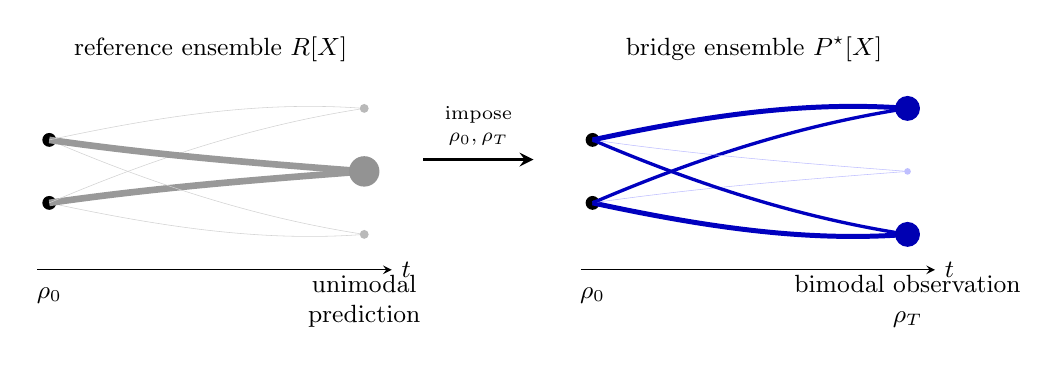
\begin{tikzpicture}[x=1cm,y=1cm,>=stealth]
    \begin{scope}
      \node[font=\small] at (2.05,1.55) {reference ensemble $R[X]$};
      \draw[->] (-0.15,-1.25) -- (4.35,-1.25) node[right,font=\small] {$t$};
      \node[font=\small] at (0,-1.58) {$\rho_0$};
      \node[align=center,font=\small] at (4,-1.65) {unimodal\\prediction};
      \fill[black] (0,-0.4) circle (2.5pt);
      \fill[black] (0,0.4) circle (2.5pt);
      \draw[gray!35,line width=0.2pt] (0,-0.4) .. controls (1.4,-0.7) and (2.7,-0.9) .. (4,-0.8);
      \draw[gray!80,line width=2.4pt] (0,-0.4) .. controls (1.4,-0.2) and (2.7,-0.1) .. (4,0);
      \draw[gray!35,line width=0.2pt] (0,-0.4) .. controls (1.4,0.2) and (2.7,0.6) .. (4,0.8);
      \draw[gray!35,line width=0.2pt] (0,0.4) .. controls (1.4,-0.2) and (2.7,-0.6) .. (4,-0.8);
      \draw[gray!80,line width=2.4pt] (0,0.4) .. controls (1.4,0.2) and (2.7,0.1) .. (4,0);
      \draw[gray!35,line width=0.2pt] (0,0.4) .. controls (1.4,0.7) and (2.7,0.9) .. (4,0.8);
      \fill[gray!55] (4,-0.8) circle (1.6pt);
      \fill[gray!85] (4,0) circle (5.5pt);
      \fill[gray!55] (4,0.8) circle (1.6pt);
    \end{scope}
    \draw[->,very thick] (4.75,0.15) -- (6.15,0.15);
    \node[align=center,font=\scriptsize] at (5.45,0.58) {impose\\$\rho_0,\rho_T$};
    \begin{scope}[xshift=6.9cm]
      \node[font=\small] at (2.05,1.55) {bridge ensemble $P^\star[X]$};
      \draw[->] (-0.15,-1.25) -- (4.35,-1.25) node[right,font=\small] {$t$};
      \node[font=\small] at (0,-1.58) {$\rho_0$};
      \node[align=center,font=\small] at (4,-1.65) {bimodal observation\\$\rho_T$};
      \fill[black] (0,-0.4) circle (2.5pt);
      \fill[black] (0,0.4) circle (2.5pt);
      \draw[blue!75!black,line width=1.8pt] (0,-0.4) .. controls (1.4,-0.7) and (2.7,-0.9) .. (4,-0.8);
      \draw[blue!25,line width=0.2pt] (0,-0.4) .. controls (1.4,-0.2) and (2.7,-0.1) .. (4,0);
      \draw[blue!75!black,line width=1.2pt] (0,-0.4) .. controls (1.4,0.2) and (2.7,0.6) .. (4,0.8);
      \draw[blue!75!black,line width=1.2pt] (0,0.4) .. controls (1.4,-0.2) and (2.7,-0.6) .. (4,-0.8);
      \draw[blue!25,line width=0.2pt] (0,0.4) .. controls (1.4,0.2) and (2.7,0.1) .. (4,0);
      \draw[blue!75!black,line width=1.8pt] (0,0.4) .. controls (1.4,0.7) and (2.7,0.9) .. (4,0.8);
      \fill[blue!70!black] (4,-0.8) circle (4.5pt);
      \fill[blue!25] (4,0) circle (1.2pt);
      \fill[blue!70!black] (4,0.8) circle (4.5pt);
    \end{scope}
  \end{tikzpicture}
  \caption{The Schr\"odinger bridge reweights histories already allowed by
  the reference distribution. Line thickness and endpoint-circle size represent
  probability weight. The reference predicts most mass near the center; the
  observation requires the bridge to move that weight to the two outer modes.}
  \label{fig:schrodinger-reweighting}
\end{figure}
\FloatBarrier

Equation~\eqref{eq:schrodinger-bridge} is the Schr\"odinger bridge. Both
endpoint distributions are fixed exactly; the unknown is the probability
distribution over complete histories between them.

\subsection{Entropy regularization in path space}

Assign each history a cost $C[X]$. With the endpoint marginals fixed,
entropy-regularized transport minimizes
\begin{equation}
  P^\star
  =\operatorname*{argmin}_{P:\,P_0=\rho_0,\,P_T=\rho_T}
  \left\{
    \int\mathcal D X\,P[X]C[X]
    +\varepsilon\int\mathcal D X\,P[X]\log P[X]
  \right\}.
  \label{eq:path-entropic-transport}
\end{equation}
The cost term concentrates $P$ on cheap histories; the entropy term spreads
$P$ among them. Their competition occurs entirely within the set of path
distributions having marginals $\rho_0$ and $\rho_T$.

Now define the Gibbs distribution on paths
\begin{equation}
  R[X]=\frac{1}{Z}\exp\!\left(-\frac{C[X]}{\varepsilon}\right).
  \label{eq:path-gibbs-distribution}
\end{equation}
Here $Z$ normalizes $R[X]$.
Direct substitution gives
\begin{equation}
  \int\mathcal D X\,P[X]C[X]
  +\varepsilon\int\mathcal D X\,P[X]\log P[X]
  =\varepsilon\KL(P\|R)-\varepsilon\log Z.
  \label{eq:path-entropy-kl-identity}
\end{equation}
Since $-\varepsilon\log Z$ is independent of $P$,
Eqs.~\eqref{eq:path-entropic-transport} and
\eqref{eq:schrodinger-bridge} have the same minimizer. Thus $R[X]$ is the
Gibbs representation of the path cost. No reference equation of motion is
needed.

For the discrete transport problem, a history is the single move
$x_i\to y_j$, with $P[X]=\pi_{ij}$ and $C[X]=C_{ij}$. Equation
~\eqref{eq:path-entropic-transport} reduces to
\begin{equation}
  \min_{\pi\in\Pi(a,b)}
  \left\{
    \sum_{i,j}C_{ij}\pi_{ij}
    +\varepsilon\sum_{i,j}\pi_{ij}\log\pi_{ij}
  \right\}.
  \label{eq:bridge-one-step-entropic-ot}
\end{equation}
Equations~\eqref{eq:bridge-one-step-entropic-ot} and
\eqref{eq:entropic-ot} differ only by the constant
$-\varepsilon\sum_{i,j}\pi_{ij}=-\varepsilon$. Entropic optimal transport
is therefore the one-step Schr\"odinger bridge, and Sinkhorn computes its
solution. With intermediate times, the same variational principle acts on
complete histories.

\begin{thebibliography}{99}
\raggedright

\bibitem{peyre-cuturi-2019}
G. Peyr\'e and M. Cuturi,
\emph{Computational Optimal Transport},
Foundations and Trends in Machine Learning, 11(5--6):355--607, 2019.

\bibitem{warrington-2016}
G. S. Warrington,
``Orthogonal bases for transportation polytopes applied to Latin squares,
magic squares and Sudoku boards,''
arXiv:1610.04259, 2016.

\bibitem{cuturi-2013}
M. Cuturi,
``Sinkhorn distances: Lightspeed computation of optimal transport,''
in \emph{Advances in Neural Information Processing Systems 26}, 2013.

\bibitem{sinkhorn-1964}
R. Sinkhorn,
``A relationship between arbitrary positive matrices and doubly stochastic
matrices,''
\emph{The Annals of Mathematical Statistics}, 35(2):876--879, 1964.

\bibitem{xie-2025}
F. Xie,
``Deriving the gradients of some popular optimal transport algorithms,''
arXiv:2504.08722v3, 2025.

\bibitem{eisenberger-2022}
M. Eisenberger, A. Toker, L. Leal-Taix\'e, F. Bernard, and D. Cremers,
``A unified framework for implicit Sinkhorn differentiation,''
in \emph{Proceedings of the IEEE/CVF Conference on Computer Vision and
Pattern Recognition}, pages 509--518, 2022.

\bibitem{jko-1998}
R. Jordan, D. Kinderlehrer, and F. Otto,
``The variational formulation of the Fokker--Planck equation,''
\emph{SIAM Journal on Mathematical Analysis}, 29(1):1--17, 1998.

\bibitem{cotler-rezchikov-2022}
J. Cotler and S. Rezchikov,
``Renormalization group flow as optimal transport,''
\emph{Physical Review D}, 108:025003, 2023.

\bibitem{schrodinger-1931}
E. Schr\"odinger,
``\"Uber die Umkehrung der Naturgesetze,''
\emph{Sitzungsberichte der Preussischen Akademie der Wissenschaften,
Physikalisch-Mathematische Klasse}, pages 144--153, 1931.

\bibitem{leonard-2014}
C. L\'eonard,
``A survey of the Schr\"odinger problem and some of its connections with
optimal transport,''
\emph{Discrete and Continuous Dynamical Systems A}, 34(4):1533--1574, 2014.

\end{thebibliography}

\end{document}
